\documentclass[UTF8,a4paper,twoside]{article}
\usepackage[UTF8]{ctex}  % 加载ctex包,支持中文
\usepackage{pdfpages}
\usepackage{tocvsec2}

% 设置参考文献
% 引入natbib包,参考文献格式相关
\usepackage[sectionbib]{natbib}
\usepackage{chapterbib}						
% 引入chapterbib包,可以分章节显示参考文献,且参考文献编号各自独立
% 参考文献格式
\usepackage{gbt7714}
% 封面信息
\newcommand{\stuname}{张三}			 	  % 学生姓名
\newcommand{\stuid}{3210xxxxxx}		  		 % 学生学号
\newcommand{\teaname}{李四}		    	  % 指导教师
\newcommand{\stugrade}{2021级}			 		% 学生年级
\newcommand{\stumajor}{信息工程} 	 		% 学生专业
\newcommand{\stucollege}{信息与电子工程学院} 		% 学生所在学院
\newcommand{\stutitle}{毕业设计题目}		% 毕设题目
\newcommand{\stuengtitlelineone}{The First Line of Your English Title}			% 毕设英文题目
\newcommand{\stuengtitlelinetwo}{The Second Line of Your English Title}

% 页面设置
% A4纸张大小 上下左边边距参考Word中"适中"类型
% A4纸张宽21cm 高29.7cm
\usepackage{geometry}	
\geometry{left=1.91cm, right=1.91cm, top=2.54cm, bottom=2.54cm}
\usepackage{subfigure}  % 导入subfigure宏包
% 设置首行缩进2字符
% 使用 \noindent 命令可以取消缩进
\usepackage{indentfirst}
\setlength{\parindent}{2em}


% 字体设置
\usepackage{fontspec}
\usepackage{amsfonts}
\usepackage{amsmath,amssymb,bm}
\usepackage{upgreek}
\usepackage{pifont}
\setmainfont[Path=fonts/, BoldFont=timesbd.ttf]{times.ttf}					% 缺省英文字体为Times New Roman
\setCJKmainfont[Path=fonts/, BoldFont=SimFangBold.ttf]{SimFang.ttf}			% 缺省中文字体为 仿宋
\setCJKfamilyfont{fs}[Path=fonts/, BoldFont=SimFangBold.ttf]{SimFang.ttf}
\newcommand{\zhengwen}{\CJKfamily{fs}\zihao{-4}}	% 正文字体 仿宋小4号
\setCJKfamilyfont{Heiti}[Path=fonts/, BoldFont=SimHeiBold.ttf]{SimHei.ttf}
\newcommand{\cover}{\CJKfamily{fs}\zihao{3}}
\setCJKfamilyfont{Songti}[Path=fonts/, BoldFont=SimSunBold.ttf]{SimSun.ttc}
\newcommand{\header}{\CJKfamily{Songti}\zihao{-5}}
\newcommand{\imageortable}{\CJKfamily{Songti}\zihao{5}}

% 行距设置
\usepackage{setspace}
\linespread{1.625}\selectfont		% 1.5倍字号,这与word中的1.5倍行距有一点差别

% 多级标题设置
\usepackage{titlesec}
\setcounter{secnumdepth}{4}		% 设置标题层次共4层
\titleformat{\section}[block]{\zihao{3}\bfseries}{\chinese{section}、}{0pt}{}
\titleformat{\subsection}[block]{\zihao{3}\bfseries}{\arabic{subsection}}{0.5em}{}
\titleformat{\subsubsection}[block]{\zihao{-3}\bfseries}{\arabic{subsection}.\arabic{subsubsection}}{0.5em}{}
\titleformat{\paragraph}{\zihao{4}\bfseries}{\arabic{subsection}.\arabic{subsubsection}.\arabic{paragraph}}{0.5em}{}
% 设置段间距
\titlespacing{\section}{0pt}{12pt}{6pt}				% 标题1 段前12磅 段后6磅
\titlespacing{\subsection}{0pt}{13pt}{13pt}			% 标题2 段前13磅 段后13磅
\titlespacing{\subsubsection}{0pt}{13pt}{13pt}		% 标题3 段前13磅 段后13磅
\titlespacing{\paragraph}{0pt}{13pt}{13pt}			% 标题4 段前13磅 段后13磅

% 定义一个新的引用命令,自动将引用放到文本的上方
\newcommand{\upcite}[1]{\textsuperscript{\citep{#1}}}

% 插入图片宏包
% 多个浮动体连续排布用参数H进行固定,如下所示,不用H会出现难以预料的排布
% \begin{figure}[H]
% content...
% \end{figure}
\usepackage{graphicx}
\usepackage{subfigure}
\usepackage{caption}
\usepackage{float}
\captionsetup{labelsep=quad,labelfont=bf,font=singlespacing}
% \renewcommand{\thefigure}{\arabic{subsection}.\arabic{figure}}
% \renewcommand{\theequation}{\arabic{subsection}.\arabic{equation}}  % 公式的编号格式
% 插入表格宏包
\usepackage{booktabs}
\usepackage{longtable}
\usepackage{multirow}
\usepackage{array}
\renewcommand{\thetable}{\arabic{subsection}.\arabic{table}}
\usepackage{enumerate}

\usepackage{caption}

% 设置图表标题字体

\renewcommand{\figurename}{\imageortable\bfseries 图}
\renewcommand{\tablename}{\imageortable\bfseries 表}

% 设置目录
\usepackage{titletoc}
\setcounter{tocdepth}{3}
\renewcommand{\thesection}{\CJKfamily{Heiti}\chinese{section}、}
\renewcommand{\thesubsection}{\arabic{subsection}}
\renewcommand{\thesubsubsection}{\arabic{subsection}.\arabic{subsubsection}}
\renewcommand{\theparagraph}{\arabic{subsection}.\arabic{subsubsection}.\arabic{paragraph}}
\titlecontents{section}[2em]{\CJKfamily{Heiti}\bfseries\zihao{-4}}{\contentslabel{2em}}{}{\titlerule*[0.5pc]{$\cdot$}\contentspage}
\titlecontents{subsection}[2.5em]{\bfseries\zihao{-4}}{\contentslabel{1em}}{}{\titlerule*[0.5pc]{$\cdot$}\contentspage}
\titlecontents{subsubsection}[4.5em]{\zihao{-4}}{\contentslabel{1.83em}}{}{\titlerule*[0.5pc]{$\cdot$}\contentspage}
\titlecontents{paragraph}[5.5em]{\zihao{-4}}{\contentslabel{2.67em}}{}{\titlerule*[0.5pc]{$\cdot$}\contentspage}
% 超链接
% colorlinks=true 超链接以颜色表示 false 超链接以方框框出
% linkcolor 指定颜色
% CJKbookmarks 让链接支持中文
\usepackage[colorlinks=true,linkcolor=black,citecolor=black,CJKbookmarks=true]{hyperref}
\newcommand{\myeqref}[1]{式 (\ref{#1})}
\newcommand{\mytaref}[1]{表 \ref{#1}}
\newcommand{\myfiref}[1]{图 \ref{#1}}
% 修改 algorithm 环境的标题为“算法”
% 直接重新定义 algorithm 的标题为中文
% 设置页眉页脚
\usepackage{fancyhdr}
\pagestyle{fancy}
\fancypagestyle{Index}{
	\setcounter{page}{1}\pagenumbering{Roman}
	\fancyhead[LO]{}
	\fancyhead[RO]{\header \stutitle}
	\fancyhead[LE]{\header 浙江大学本科生毕业论文(设计)}
	\fancyhead[RE]{}
	\fancyfoot[C]{\zihao{-5} \thepage}
}
\fancypagestyle{Require}{
    \fancyhead[L]{}
	\fancyhead[R]{\header \stutitle}
    \fancyfoot[C]{} % 清空页脚的页码
}
\fancypagestyle{Content}{
	\setcounter{page}{1}\pagenumbering{arabic}
	\fancyhead[LO]{}
	\fancyhead[RO]{\header \stutitle}
	\fancyhead[LE]{\header 浙江大学本科生毕业论文(设计)}
	\fancyhead[RE]{}
	\fancyfoot[C]{\zihao{-5} \thepage}
}

% 插入公式
\usepackage{amsmath}
\usepackage{indentfirst}
\usepackage{algorithm}
\usepackage{algpseudocode}

\numberwithin{equation}{subsection} % 将公式编号与章节关联
\numberwithin{figure}{subsection} % 图的编号与章节关联
\numberwithin{table}{subsection}  % 表的编号与章节关联
\renewcommand{\contentsname}{\vspace{-\baselineskip}}											
% 这条命令可以控制引入编译的各子文件是否参与编译	

\begin{document}
    % 封面
    \pagestyle{empty}

\begin{center}
 \vspace*{5ex}
 
\includegraphics[width=11cm]{images/zju.jpg} 
  
 \vspace{1ex}
        {\CJKfamily{Heiti}\zihao{-1}\bfseries
 本\ \ 科\ \ 生\ \ 毕\ \ 业\ \ 论\ \ 文(设计)
  
 \vspace{15pt}
 文献综述和开题报告}
  
 \vspace{50pt}
 
\includegraphics[width=70pt]{images/qsy.jpg}
 
 \cover 
 \vspace{24pt}
        \makebox[1.6cm][l]{\bfseries 题目}\underline{\makebox[14.9cm]{\textbf{\stutitle}}}
        \makebox[2.5cm][l]{\bfseries 英文题目}\underline{\makebox[14cm]{\zihao{4}\textbf{\stuengtitlelineone}}}
        \makebox[2.5cm][l]{}\underline{\makebox[14cm]{\zihao{4}\textbf{\stuengtitlelinetwo}}}
        \vspace{40pt}
        
 \makebox[3.2cm][l]{\bfseries 姓名与学号}\underline{\makebox[7cm]{\stuname\quad \stuid}}
 
 \vspace{20pt}
 \makebox[3.2cm][l]{\bfseries 指导教师}\underline{\makebox[7cm]{\teaname}}
 
 \vspace{20pt}
 \makebox[3.2cm][l]{\bfseries 年级与专业}\underline{\makebox[7cm]{\stugrade\quad\stumajor}}
 
 \vspace{20pt}
 \makebox[3.2cm][l]{\bfseries 所在学院}\underline{\makebox[7cm]{\stucollege}}
 
 \vspace{16ex}
\end{center}\newpage\thispagestyle{empty}\ 
    % 要求
    \newpage
    \pagestyle{Require}
    \pagestyle{Require}
\noindent{\zihao{4}\bfseries 一、题目:}\zihao{4}\stutitle \\
{\zihao{4}\bfseries 二、指导教师对文献综述、开题报告、外文翻译的具体要求}



\vfill
{\hfill {\zihao{4}\bfseries 指导教师(签名)\underline{\makebox[3cm]{}}}}\par
\hfill {\zihao{4}  2024年11月4日}\newpage\thispagestyle{empty}\ 
	
    % 目录
    \newpage
    \pagestyle{Index}
    \begin{center} {\bfseries \zihao{3}目录}
    \end{center}
    \tableofcontents
    \noindent {\CJKfamily{Heiti}\zihao{-4}\bfseries \hspace{0.36em}毕业论文(设计)文献综述和开题报告考核}
    \newpage 
	\ \\ 
    % 正文
    \newpage
    \cleardoublepage\pagestyle{Content}\zhengwen
\section{文献综述}
    
\subsection{背景介绍}
这是\LaTeX。
		
\noindent 测试测试
	
\subsubsection{公式}
公式见\myeqref{eq:1}
\begin{equation}
\label{eq:1}
a^2 + b^2 = c^2
\end{equation}
	
\paragraph{图片}

图片见\myfiref{Wallpaper}
\vspace{10ex}
\begin{figure}[H]
	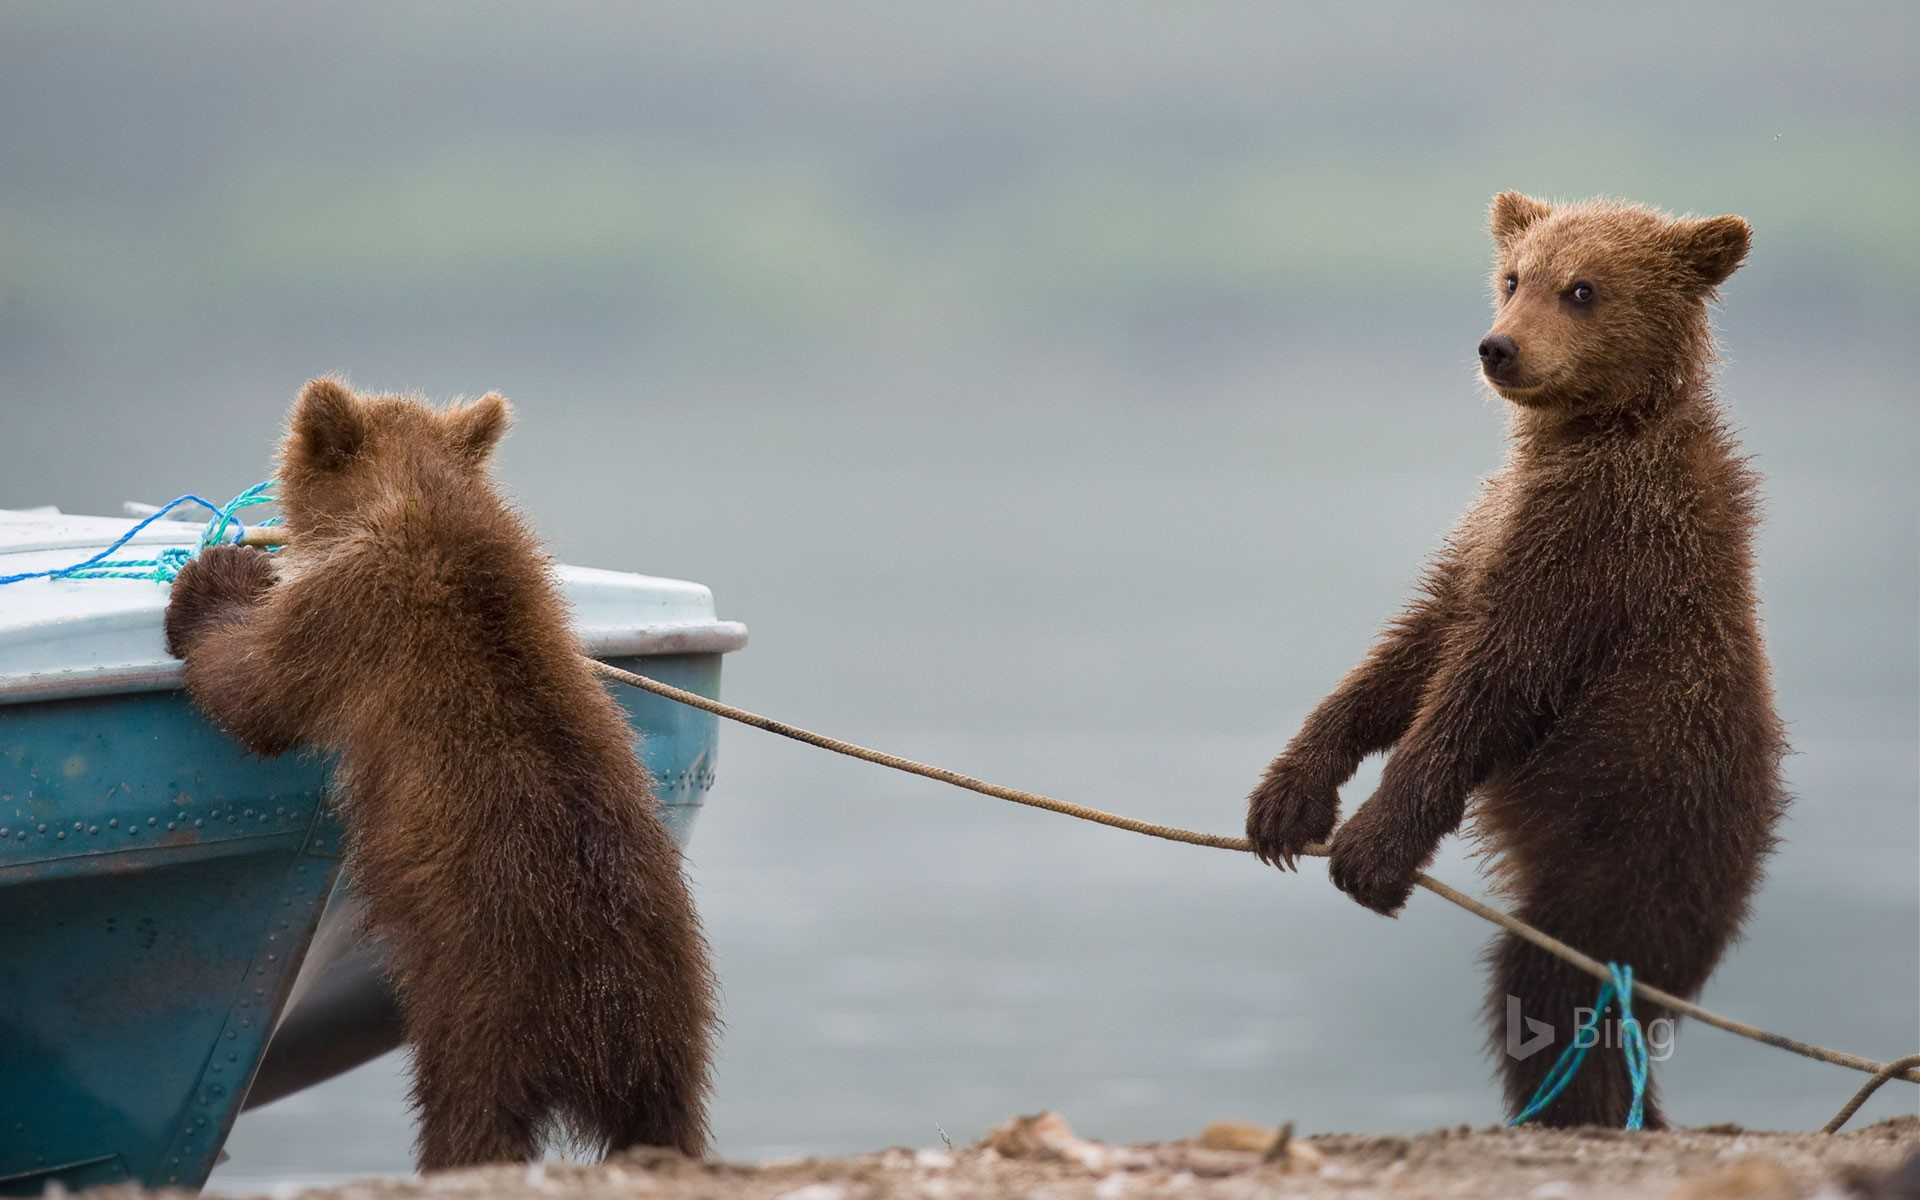
\includegraphics[width=\textwidth]{images/BingWallpaper-2019-04-01.jpg}
	\caption{\imageortable\bfseries 第一张图}
    \label{Wallpaper}
\end{figure}


\begin{table}
    \centering\imageortable
    \renewcommand{\arraystretch}{1.5}
    \caption{\imageortable\bfseries 测试}
    \begin{tabular}{>{\centering\arraybackslash}p{1.5cm}>{\centering\arraybackslash}p{1.5cm}>{\centering\arraybackslash}p{1.5cm}>{\centering\arraybackslash}p{1.5cm}}\hline
        标题1 & 标题2 & 标题3 & 标题4\\ \hline
        111 & 一个测试 & $a$ & $a+b$\\
        222 &  &  & \\
        333 &  &  & \\ \hline 
    \end{tabular}
    \label{tab:my_label}
\end{table}

参考文献\upcite{何祚镛2007近场声全息技术应用有关物理问题研究}的引用。

\subsection{国内外研究现状}
\begin{equation}
    y(x)=y_0+\int_{x_0}^xf(t,y(t))\text{d}t
\end{equation}
\subsubsection{研究方向及进展}
	
\subsubsection{存在问题}
	
\subsection{研究展望}

\bibliographystyle{gbt7714-numerical}
\phantomsection		% 要想目录中参考文献的超链接正确需要加这一语句
\subsection{参考文献}
{\normalfont\CJKfamily{Songti}\zihao{5}\setlength{\baselineskip}{14pt}
\renewcommand{\refname}{\vspace{-\baselineskip}}
\bibliography{reference/refs}}
    \cleardoublepage
    
\section{开题报告}

\subsection{问题提出的背景}

\subsubsection{背景介绍}
引用\upcite{schweizer2013comparative}

\paragraph{段的标题}

\subsubsection{本研究的意义和目的}

\subsection{论文的主要内容和技术路线}

\subsubsection{主要研究内容}

\subsubsection{技术路线}

\subsubsection{可行性分析}

\subsection{研究计划进度安排及预期目标}

\subsubsection{进度安排}

\subsubsection{预期目标}

% 参考文献
\newpage
\bibliographystyle{gbt7714-numerical}
\phantomsection		% 要想目录中参考文献的超链接正确需要加这一语句
\subsection{参考文献}
{\normalfont\CJKfamily{Songti}\zihao{5}\setlength{\baselineskip}{14pt}
\renewcommand{\refname}{\vspace{-\baselineskip}}
\bibliography{reference/refs}}
    \addtocontents{toc}{\protect\setcounter{tocdepth}{1}}
    \cleardoublepage
\section{外文翻译}
\renewcommand{\theequation}{\arabic{equation}}
\renewcommand{\thefigure}{\arabic{figure}}
\begin{center}
    \zihao{3}\textbf{论文题目}
\end{center}
\subsection*{摘要}
这是摘要。
\settocdepth{part} % 以下部分不计入目录


% 注:正文部分的subsection中公式和图表的编号会在每一个subsection中重新开始计数,如果需要在整个文档中保持编号的连续性,可以在每个subsection后加上以下两行代码:
% \setcounter{equation}{上一个subsection中最后一个公式的编号}
% \setcounter{figure}{上一个subsection中最后一个图表的编号}

\subsection{引言}
这是引言,测试参考文献\cite{schweizer2013comparative}。

% 参考文献
\newpage
\bibliographystyle{gbt7714-numerical}
\phantomsection		% 要想目录中参考文献的超链接正确需要加这一语句
\subsection{参考文献}
{\normalfont\CJKfamily{Songti}\zihao{5}\setlength{\baselineskip}{14pt}
\renewcommand{\refname}{\vspace{-\baselineskip}}
\bibliography{reference/refs}}

\resettocdepth % 恢复目录计数
    \cleardoublepage\section{外文原文}

    % 考核表
    \newpage
    \cleardoublepage\pagestyle{empty}\bfseries
\begin{center}
    \zihao{-2} 毕业论文(设计)文献综述和开题报告考核
\end{center}
% 将该标题加入目录(在章节中插入)
% \addcontentsline{toc}{section}{\hspace{-2.2em} 毕业论文(设计)文献综述和开题报告考核}
\ \\
\zihao{4}对文献综述、外文翻译和开题报告评语及成绩评定
\vfill


\begin{flushright}
\begin{table}[!htbp]
    \renewcommand{\arraystretch}{3.5}  % 调整行高,可以增大或减小数值
    \hfill
    \begin{tabular}{|>{\centering\arraybackslash}m{3cm}|>{\centering\arraybackslash}m{2.5cm}|>{\centering\arraybackslash}m{2.5cm}|>{\centering\arraybackslash}m{2.5cm}|} \hline
        \bfseries\zihao{4}成绩比例 & \bfseries\zihao{5}文献综述占(10\%) & \bfseries\zihao{5}开题报告占(15\%)& \bfseries\zihao{5}外文翻译占(5\%)\\ \hline
        \bfseries\zihao{4}分值 &  &  & \\ \hline
    \end{tabular}
\end{table}  
{\hfill {\zihao{-4}\bfseries 开题报告答辩小组负责人(签名)\underline{\makebox[3cm]{}}}}\\
\hfill {\zihao{-4}  2025年\quad\quad  月\quad\quad  日}
\end{flushright} 
	
			
\end{document}